\subsection{Event selection} \label{sec:Charmonia_Analysis_Selection}

The charmonium candidates are reconstructed in the dimuon decay channel (i.e. \JPsiToMuMu and \PsiPToMuMu), by pairing opposite-charge muons. Since the \JPsi and \PsiP masses are small ($\text{m}_{\JPsi} = 3.097~\GeVcc$ and $\text{m}_{\PsiP} = 3.686~\GeVcc$), the signal events are dominated by the presence of low \pt muons ($\langle\pt^{\PGm}\rangle \sim 1.6~\GeVc$), contrary to the \PW-boson analysis reported in \chp{sec:WBoson}. The selection used to identify the charmonium events is detailed in this section.

%%------------------------------------------------------------%%
\subsubsection{Minimum bias event selection} \label{sec:Charmonia_Analysis_Selection_EventFilter}

The \Runpp and \RunPbPb minimum bias events are selected by applying a global event filter (GEF) offline to suppress the background events not originating from the inelastic hadronic scattering. The GEF for \Runpp collision events consists of the following filters:
\begin{itemize}
\item Beam-Scraping filter: Requires at least 25$\%$ of tracks in the event to be high quality tracks.
\item Primary Vertex filter: Requires a primary vertex reconstructed from at least two tracks, within a longitudinal (transverse) distance of \SI{25}{\cm} (\SI{2}{\cm}) of the IP.
\end{itemize}

In the case of \RunPbPb collisions, since the projectiles are more charged (82 protons per \Pb ion), the background contribution from electromagnetic interactions between \Pb beams is significantly enhanced, and as a result a tighter event selection is applied including the following filters:

\begin{itemize}
 \item HF coincidence filter: requires at least three towers on each side of the interaction point in the HF calorimeter, with an energy deposit per tower of at least \SI{3}{\GeV}. This filter rejects events from electronic noise and beam-beam electromagnetic interactions.
 \item Cluster compatibility filter: rejects beam-scrapping events (i.e. muons produced when the beam particles hit the LHC collimators), by requiring that the shape of the silicon pixel clusters are compatible with tracks originating from the primary vertex.
\end{itemize}

The \RunPbPb collision events are also required to contain at least one reconstructed primary vertex as done for \Runpp data. The efficiency of the GEF in \RunPbPb minimum bias events has been determined to be $99{\pm}2$\%. This  efficiency can surpass 100\% due to the remaining contamination of non-hadronic collisions in the sample. The number of \RunPbPb minimum bias events passing the GEF corresponds to $N_{\text{MB}} = 2.34 \times 10^{9}$ for HIOniaDoubleMu0 and $N_{\text{MB}} = 3.09 \times 10^{9}$ for HIOniaPeripheral30100.

%%------------------------------------------------------------%%
\subsubsection{Trigger} \label{sec:Charmonia_Analysis_Selection_Trigger}

The events used in the analysis of the charmonium production in \Runpp and \RunPbPb collisions were selected by the trigger called \verb-HLT_HIL1DoubleMu0-, which requires the presence of two L1 muons (with no muon \pt requirement) in coincidence with a bunch crossing identified by the BPTX detectors (to suppress contributions from cosmic-ray muons).

In addition, events derived from the dimuon peripheral dataset HIOniaPeripheral30100 were selected by the trigger \verb-HLT_HIL1DoubleMu0_2HF_Cent30100-, which requires, in addition to the \verb-HLT_HIL1DoubleMu0- trigger conditions, a signal in coincidence on both sides of the HF detector and a total energy deposit in the HF calorimeters consistent with a collision centrality between 30\% and 100\%.

To make sure that each muon employed in the analysis is associated to an online muon that fired the dimuon triggers, the reconstructed muons are required to be matched to the corresponding L1 muons within a $\eta$-$\phi$ cone defined as:

\begin{equation}
 \Delta{R}\left(\PGm_{\text{reco}} , \PGm_{\text{L1}}\right) = \sqrt{\left( \left(\eta_{\text{reco}} - \eta_{\text{L1}}\right)^{2} +  \left(\phi_{\text{reco}} - \phi_{\text{L1}}\right)^{2} \right)} < 0.3
\end{equation}

The standard $\Delta{R}<0.3$ threshold is employed in CMS analyses using L1 muon triggers~\cite{CMSTrigger}. Since L1 muons are reconstructed only in the muon stations, their position ($\eta$, $\phi$) resolution is worse than for HLT L3 muons (which includes also the inner-tracker information). As a consequence, a wider $\Delta{R}$ matching criteria is utilised for L1 muons compared to the one used in the \PW-boson analysis ($\Delta{R}<0.1$).

%%------------------------------------------------------------%%

\subsubsection{Centrality determination in \RunPbPb collisions}

The centrality percentiles of \RunPbPb collisions are derived by sampling the distribution of the total energy deposited in the HF calorimeters in bins of 0.5\% of the total hadronic cross section. The HF energy distribution is determined in minimum-bias events (i.e. requiring a bunch crossing and a coincidence between signals from the $-z$ and $+z$ sides of the HF calorimeters) passing the GEF. The yield as a function of the HF energy is then corrected for the efficiency of the minimum-bias trigger and the GEF selection. \fig{fig:energyHF} presents the distribution of the total HF energy in \RunPbPb collisions separated in centrality classes.

\begin{figure}[htb!]
 \centering
 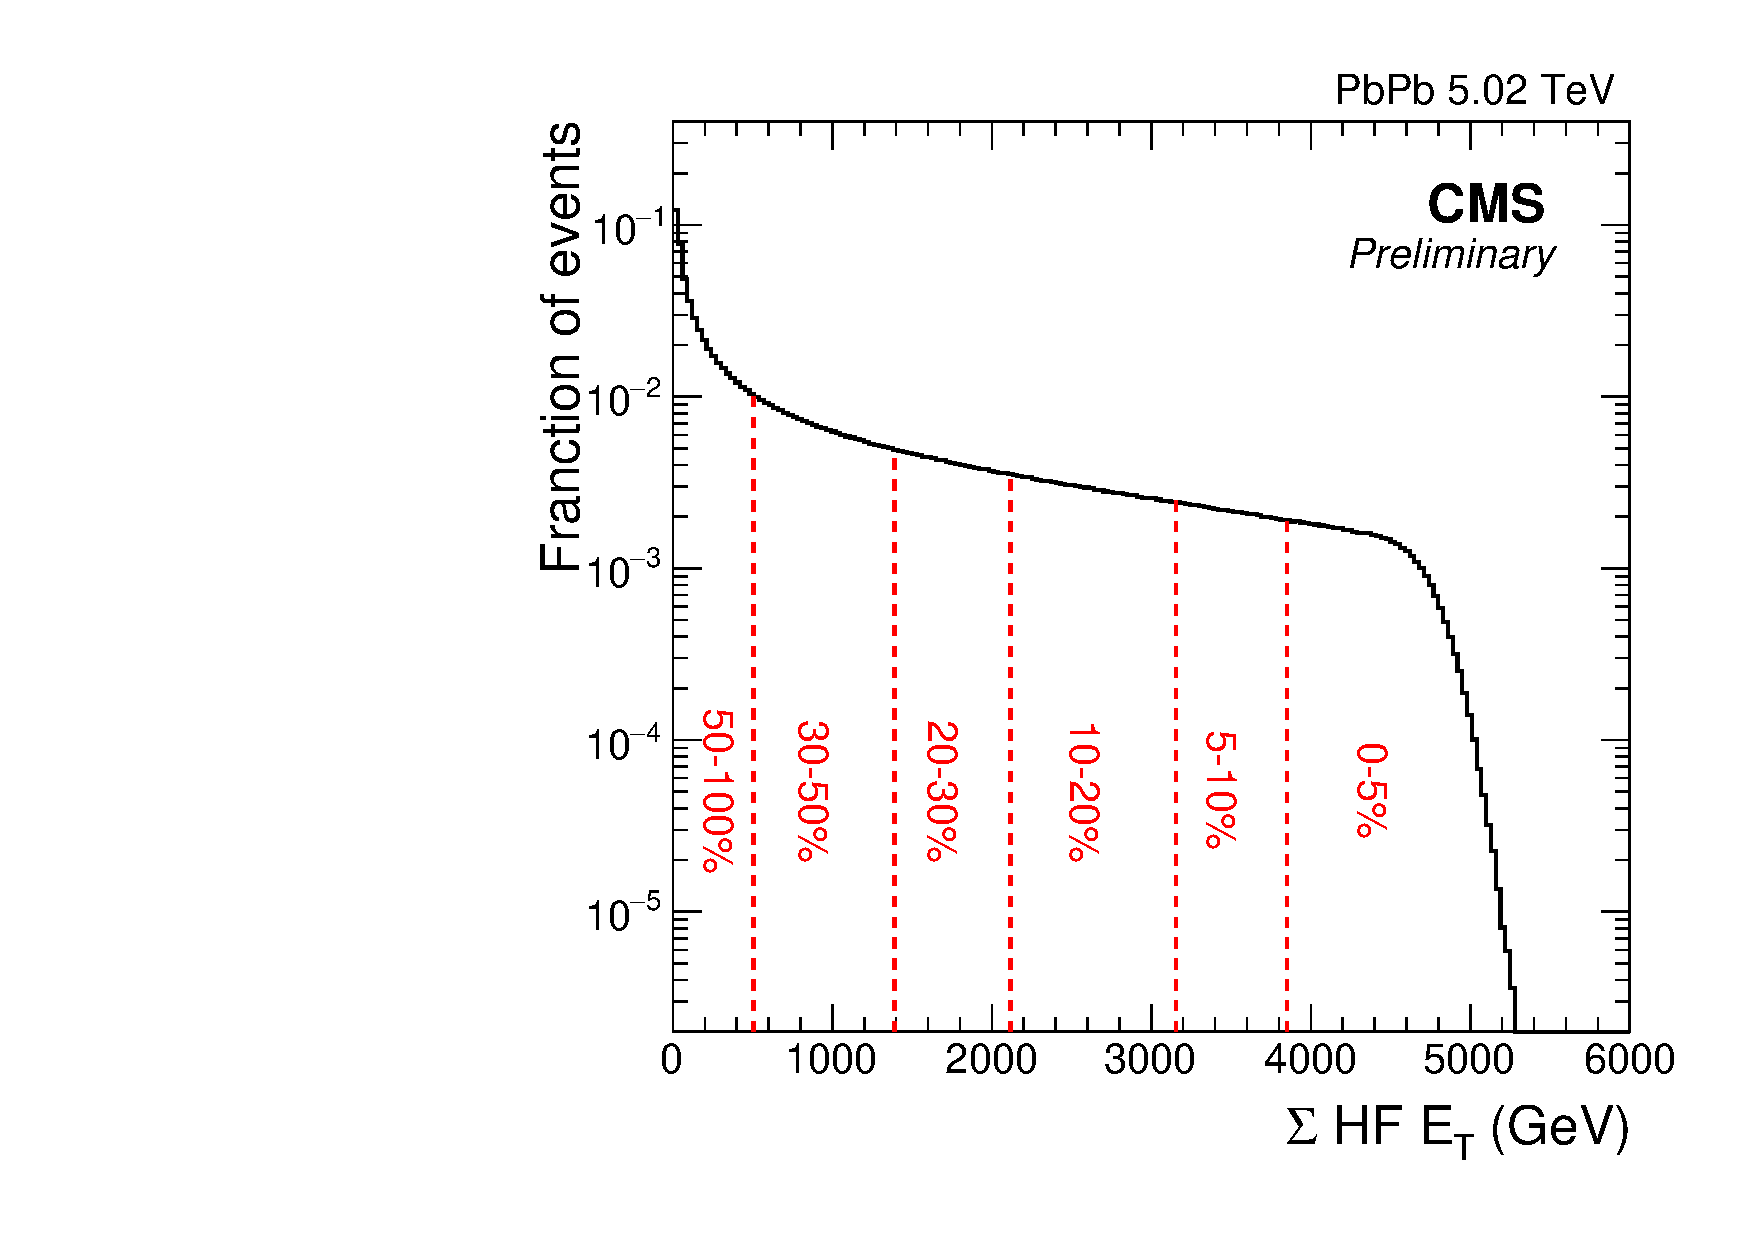
\includegraphics[width=0.55\textwidth]{Figures/Charmonia/Analysis/EventSelection/EHF.pdf}
 \caption{Distribution of the total energy deposited in the HF calorimeters in \RunPbPb collisions at \SI{5.02}{\TeV}, for minimum-bias events passing the GEF selection. The different centrality classes are shown. Figure taken from the internal analysis note~\cite{Centrality_PbPb}.}
 \label{fig:energyHF}
\end{figure}

\fig{fig:centrality} shows the centrality distribution of the dimuon triggered \RunPbPb dataset. The selection of hard-probe processes, such as the production of charmonium states, bias the centrality distribution towards central collisions. 

\begin{figure}[htb!]
 \centering
 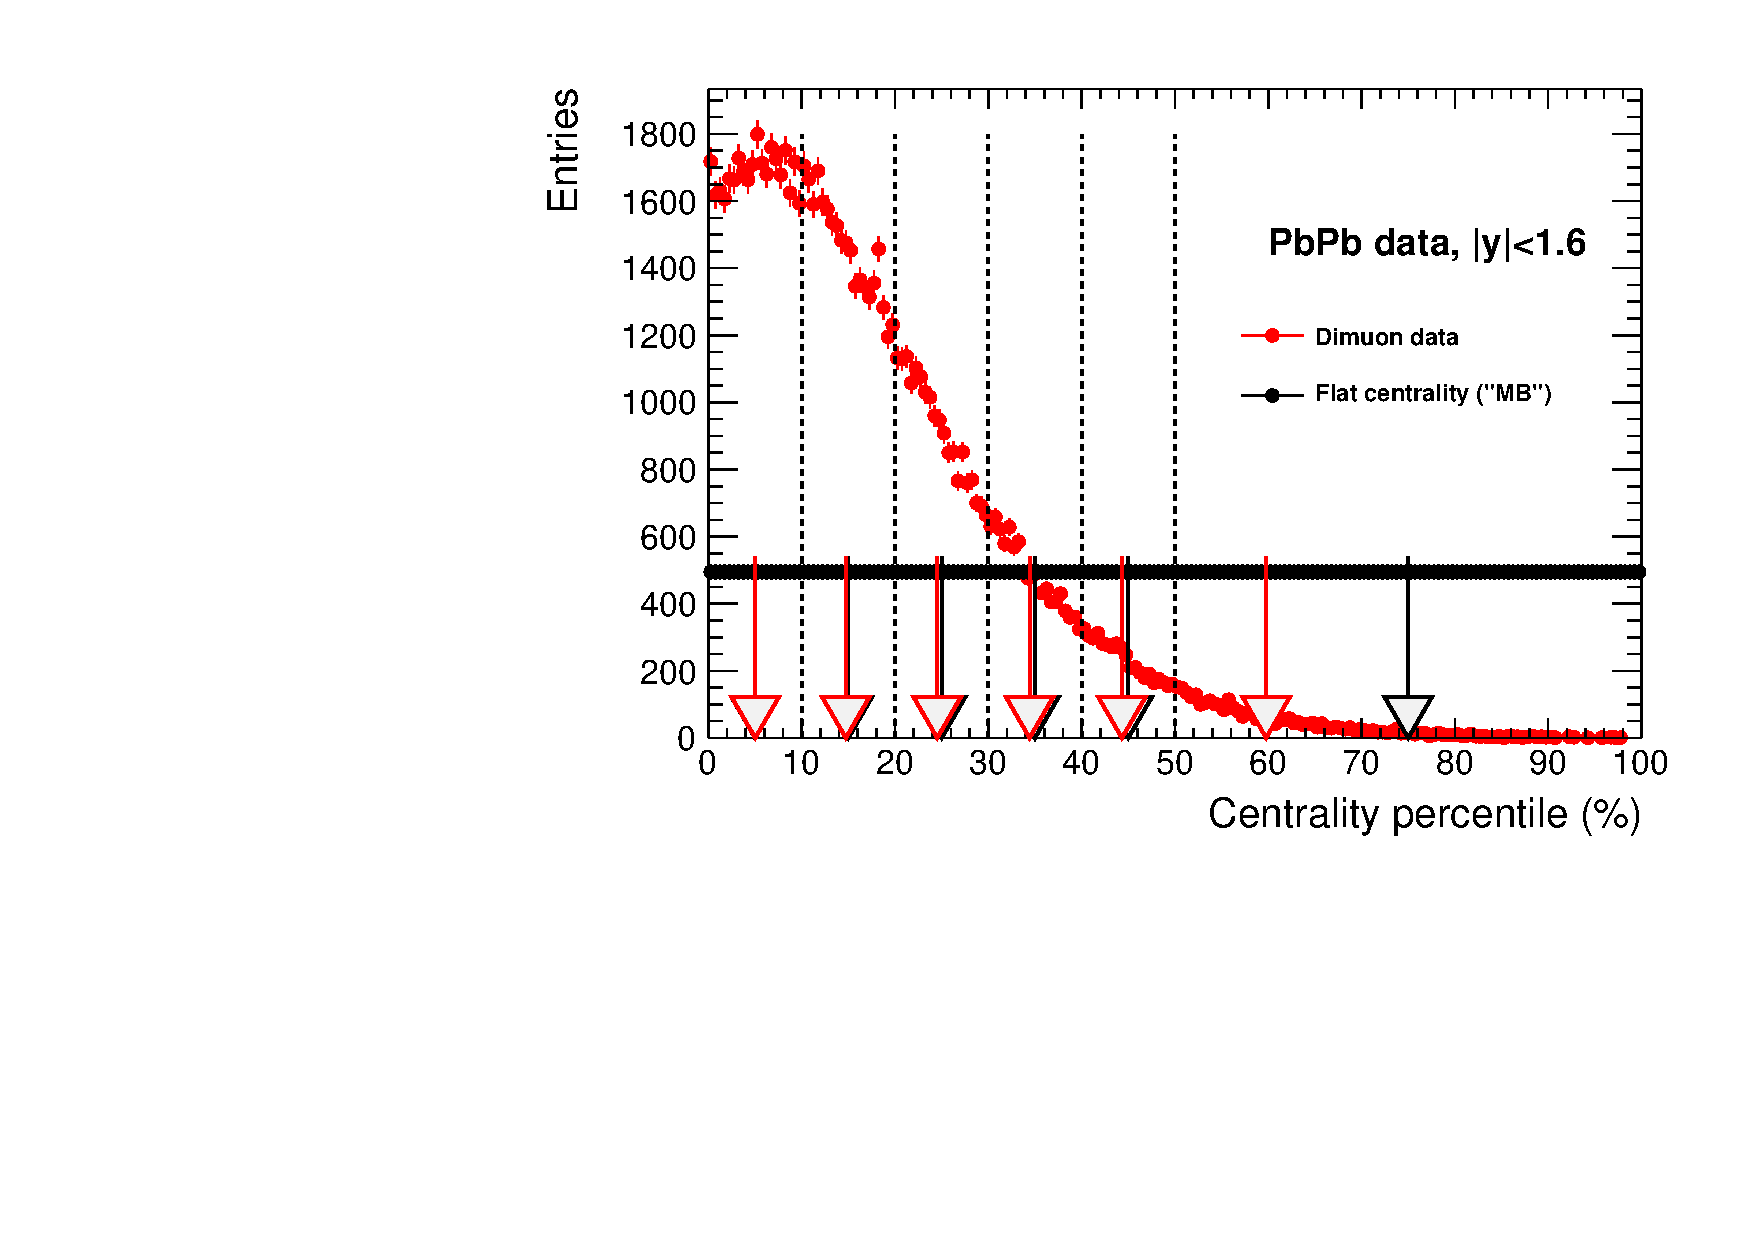
\includegraphics[width=0.45\textwidth]{Figures/Charmonia/Analysis/EventSelection/centrality_mid.pdf}
 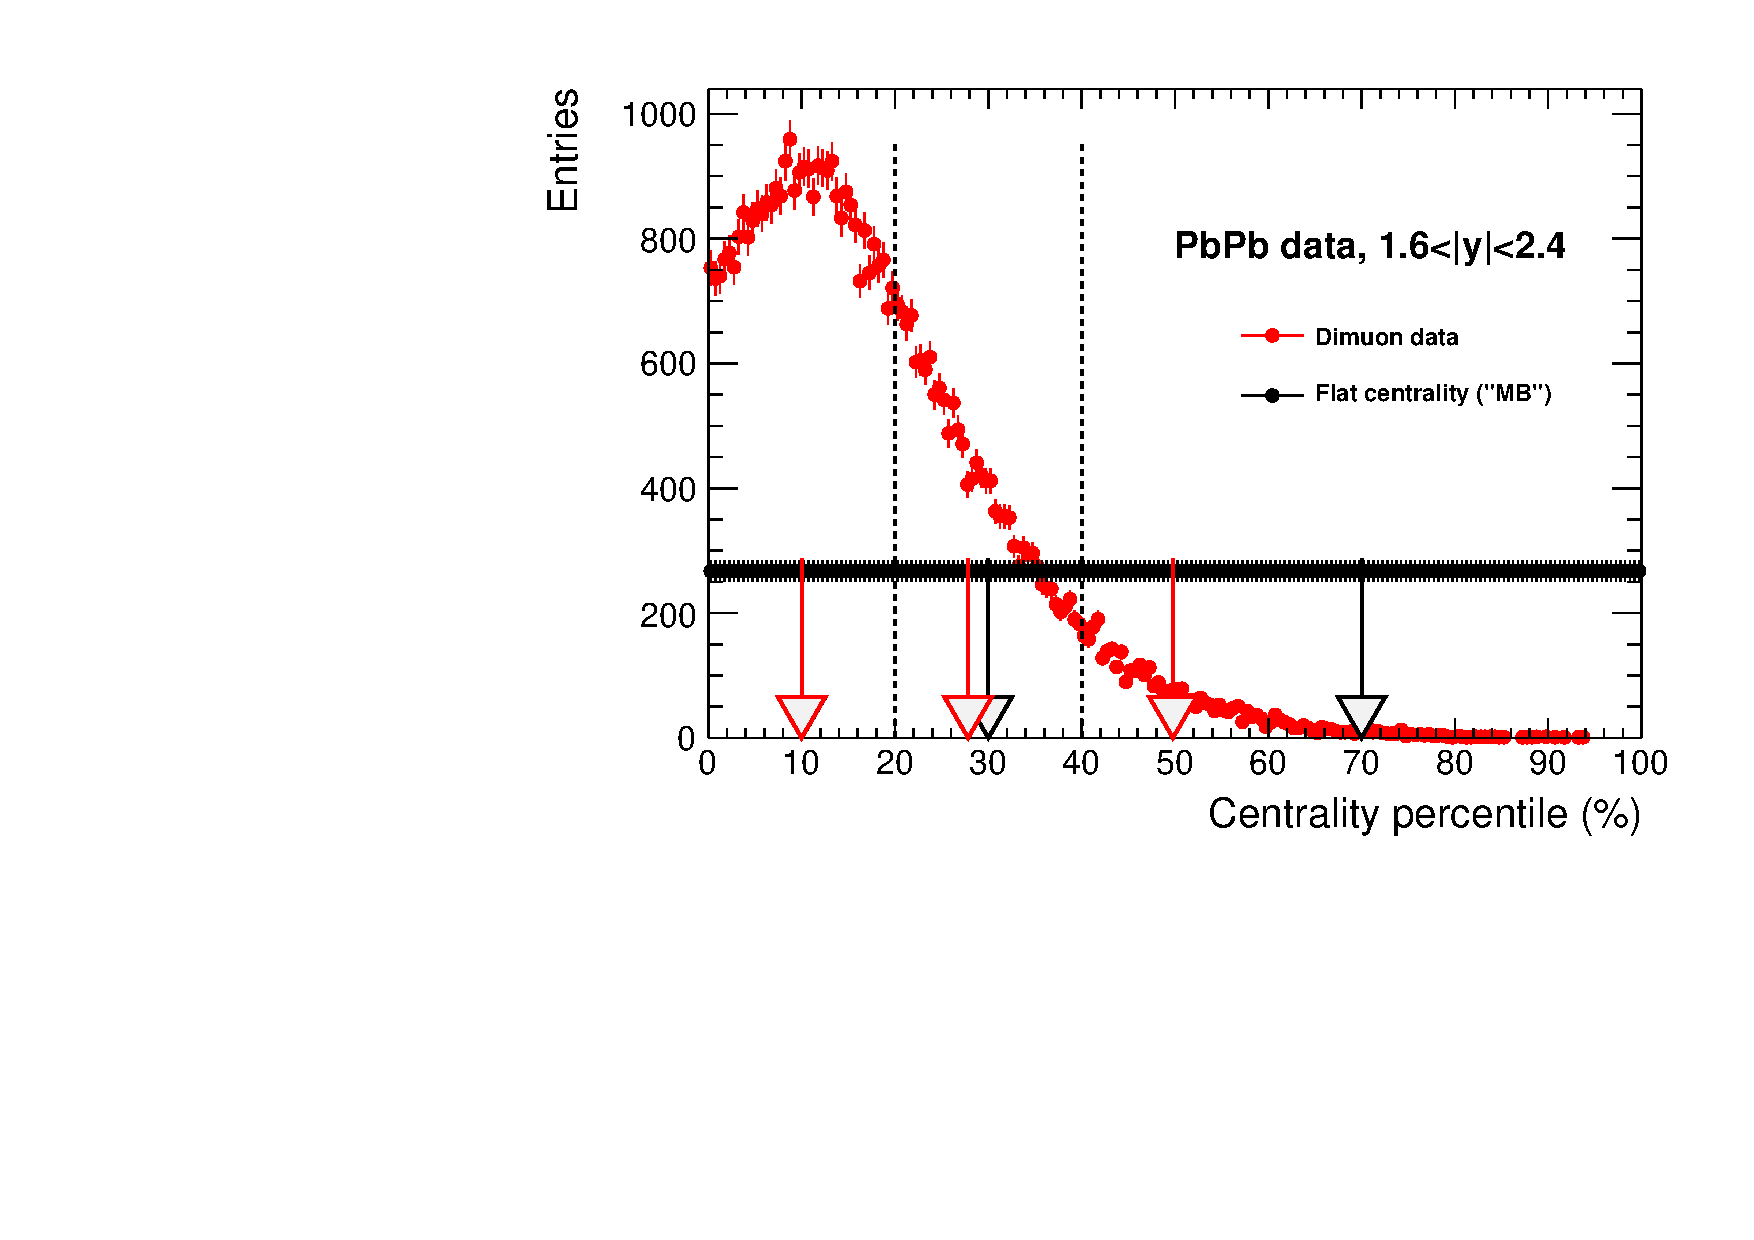
\includegraphics[width=0.45\textwidth]{Figures/Charmonia/Analysis/EventSelection/centrality_fwd.pdf}
 \caption{Centrality distribution of \mumu events in \RunPbPb collisions passing the GEF cuts (red), with $2.2<M_{\mumu}<4.5~\GeVcc$, for $|y|<1.6$ (left) and $1.6<|y|<2.4$ (right). The distribution of the minimum-bias sample, flat by definition, is shown in black. The limits of the centrality bins used for the \PsiP analysis are shown as vertical dashed lines, with the most central (peripheral) range on the right (left). The average centrality in each centrality range is also shown as an arrow, in red and black for the dimuon and minimum-bias datasets, respectively. 
 \label{fig:centrality}}
\end{figure}

The centrality percentiles are associated with the average geometrical quantities of the collision (e.g. \npart and \taa) using a Glauber MC model as explained in \sect{sec:Physics_HI_Glauber}. The centrality intervals used in \RunPbPb collisions and the corresponding average \npart and \taa values are presented in \tab{tab:TAAValues}.

\begin{table}[htb!]
 \centering
  \renewcommand{\arraystretch}{1.1}
 \begin{tabular}{|c|c|c|}
  \hline
  Centrality range [\%] & \avgtaa & \avgnpart \\
  \hline
  0 - 100   & $5.61 {+0.16} {-0.19}$   &   $114.0 {+2.6} {-2.6}$ \\
  \hline%\hline
  0 - 5     & $25.98 {+0.47} {-0.77}$  &   $384.3 {+1.8} {-2.0}$ \\   
  %\hline
  5 - 10    & $20.46 {+0.38} {-0.60}$  &   $333.3 {+3.0} {-3.2}$ \\   
  %\hline
  10 - 15   & $16.11 {+0.35} {-0.50}$  &   $285.4 {+3.5} {-3.7}$ \\   
  %\hline
  15 - 20   & $12.60 {+0.32} {-0.43}$  &   $242.9 {+3.8} {-3.9}$ \\   
  %\hline
  20 - 25   & $9.80 {+0.31} {-0.37}$   &   $205.7 {+3.9} {-4.1}$ \\   
  %\hline
  25 - 30   & $7.52 {+0.29} {-0.32}$   &   $172.7 {+4.0} {-4.0}$ \\   
  %\hline
  30 - 35   & $5.71 {+0.27} {-0.27}$   &   $144.1 {+4.0} {-4.0}$ \\   
  %\hline
  35 - 40   & $4.25 {+0.23} {-0.24}$   &  $118.7 {+4.0} {-4.0}$  \\   
  %\hline
  40 - 45   & $3.10 {+0.19} {-0.19}$   &   $96.51 {+3.8} {-3.8}$ \\   
  %\hline
  45 - 50   & $2.22 {+0.16} {-0.16}$   &   $77.4 {+3.7} {-3.6}$  \\   
  %\hline
  50 - 60   & $1.30 {+0.12} {-0.12}$   &   $53.9 {+3.2} {-3.1}$  \\   
  %\hline
  60 - 70   & $0.57 {+0.07} {-0.06}$   &   $30.6 {+2.6} {-2.4}$  \\   
  %\hline
  70 - 100  &  $0.11 {+0.02} {-0.01}$  &   $8.3 {+1.0} {-0.6}$   \\
  \hline%\hline
  0 - 10    & $23.22 {+0.43} {-0.69}$  &   $358.8 {+2.4} {-2.6}$ \\   
  %\hline
  10 - 20   & $14.35 {+0.33} {-0.45}$  &   $264.2 {+3.6} {-3.8}$ \\   
  %\hline
  20 - 30   & $8.66 {+0.29} {-0.33}$   &   $189.2 {+4.0} {-4.1}$ \\   
  %\hline
  30 - 40   & $4.98 {+0.24} {-0.24}$   &   $131.4 {+4.0} {-4.0}$ \\   
  %\hline
  40 - 50   & $2.66 {+0.18} {-0.17}$   &   $87.0 {+3.7} {-4.3}$  \\   
  %\hline
  50 - 100  & $0.44 {+0.05} {-0.03}$   &   $21.9 {+1.8} {-1.0}$  \\    
  \hline%\hline
  10 - 30   & $11.51 {+0.30} {-0.39}$  &   $226.7 {+3.7} {-3.9}$ \\   
  %\hline
  30 - 100  & $1.41 {+0.09} {-0.06}$   &   $46.8 {+2.4} {-1.2}$  \\
  \hline%\hline
  0 - 20    & $18.79 {+0.37} {-0.56}$  &   $311.5 {+2.9} {-3.1}$ \\   
  %\hline
  20 - 40   & $6.82 {+0.26} {-0.28}$   &   $160.3 {+4.0} {-4.0}$ \\ 
  %\hline
  40 - 100  & $0.81 {+0.07} {-0.05}$   &   $32.7 {+2.1} {-1.1}$  \\ 
  \hline
 \end{tabular}
 \caption{Values of the centrality-integrated number of participants \avgnpart and nuclear overlap factor \avgtaa, determined in the different collision centrality ranges used in the analysis. Information taken from the private Ref.~\cite{Centrality_PbPb}.}
 \label{tab:TAAValues}
\end{table}


%%------------------------------------------------------------%%
\subsubsection{Muon selection} \label{sec:Charmonia_Analysis_Selection_MuonIdentification}

Muon candidates are identified using a \textit{soft} selection. Contrary to the muon selection criteria used in the \PW-boson analysis, which was optimised for high-\pt muons, the \textit{soft} selection has been designed to be highly efficient for muons with low transverse momentum (\pt < 10~\GeVc). The \textit{soft} selection requires muon candidates to pass the following criteria:

\begin{itemize}
 \item The muon track is identified both by the tracker-muon and the global-muon algorithms.
 \item The tracker track extrapolated to the muon system is matched with at least one muon segment within a distance less than $3\sigma$ along the $x$ and $y$ coordinates. Muon segments are excluded if they have a better match with other tracker tracks.
 \item The muon track includes hits in more than five inner-tracker layers, ensuring a good \pt measurement.
 \item The muon track has measurements in at least one pixel layer to suppress muons from decays in flight.
 \item The transverse impact parameter (longitudinal distance) of the muon track is consistent with the primary vertex within \SI{0.3}{\cm} (\SI{20}{\cm}), to reduce the background from cosmic-ray muons.
\end{itemize}


%%------------------------------------------------------------%%
\subsubsection{Muon kinematic cut} \label{sec:Charmonia_Analysis_Selection_MuonKinematic}

The single muon kinematic selection is optimised, using the \JPsi-meson simulated samples, by requiring (in different muon $\pt-\eta$ bins) that the number of muon candidates passing the trigger, reconstruction and identification algorithms is more than $10\%$ of the number of generated muons. The muon kinematic cuts are described in \eq{eq:SingleMuonAccCuts} and shown in \fig{fig:SingleMuonAccEff}.

\begin{equation}
 \centering
 \setlength\arraycolsep{20pt}
 \begin{array}{l c r r}
  \pt^{\PGm}>3.5\GeVc & & \text{for}\enspace \abs{\eta^{\PGm}}<1.2 & \\
  \pt^{\PGm}>(5.77 - 1.89\times\abs{\eta^{\PGm}})\GeVc & &  \text{for}\enspace 1.2\le\abs{\eta^{\PGm}}<2.1 &\\
  \pt^{\PGm}>1.8\GeVc & & \text{for}\enspace 2.1\le\abs{\eta^{\PGm}}<2.4 &
 \end{array}
 \label{eq:SingleMuonAccCuts}
\end{equation}

\begin{figure}[htb!]
 \centering 
  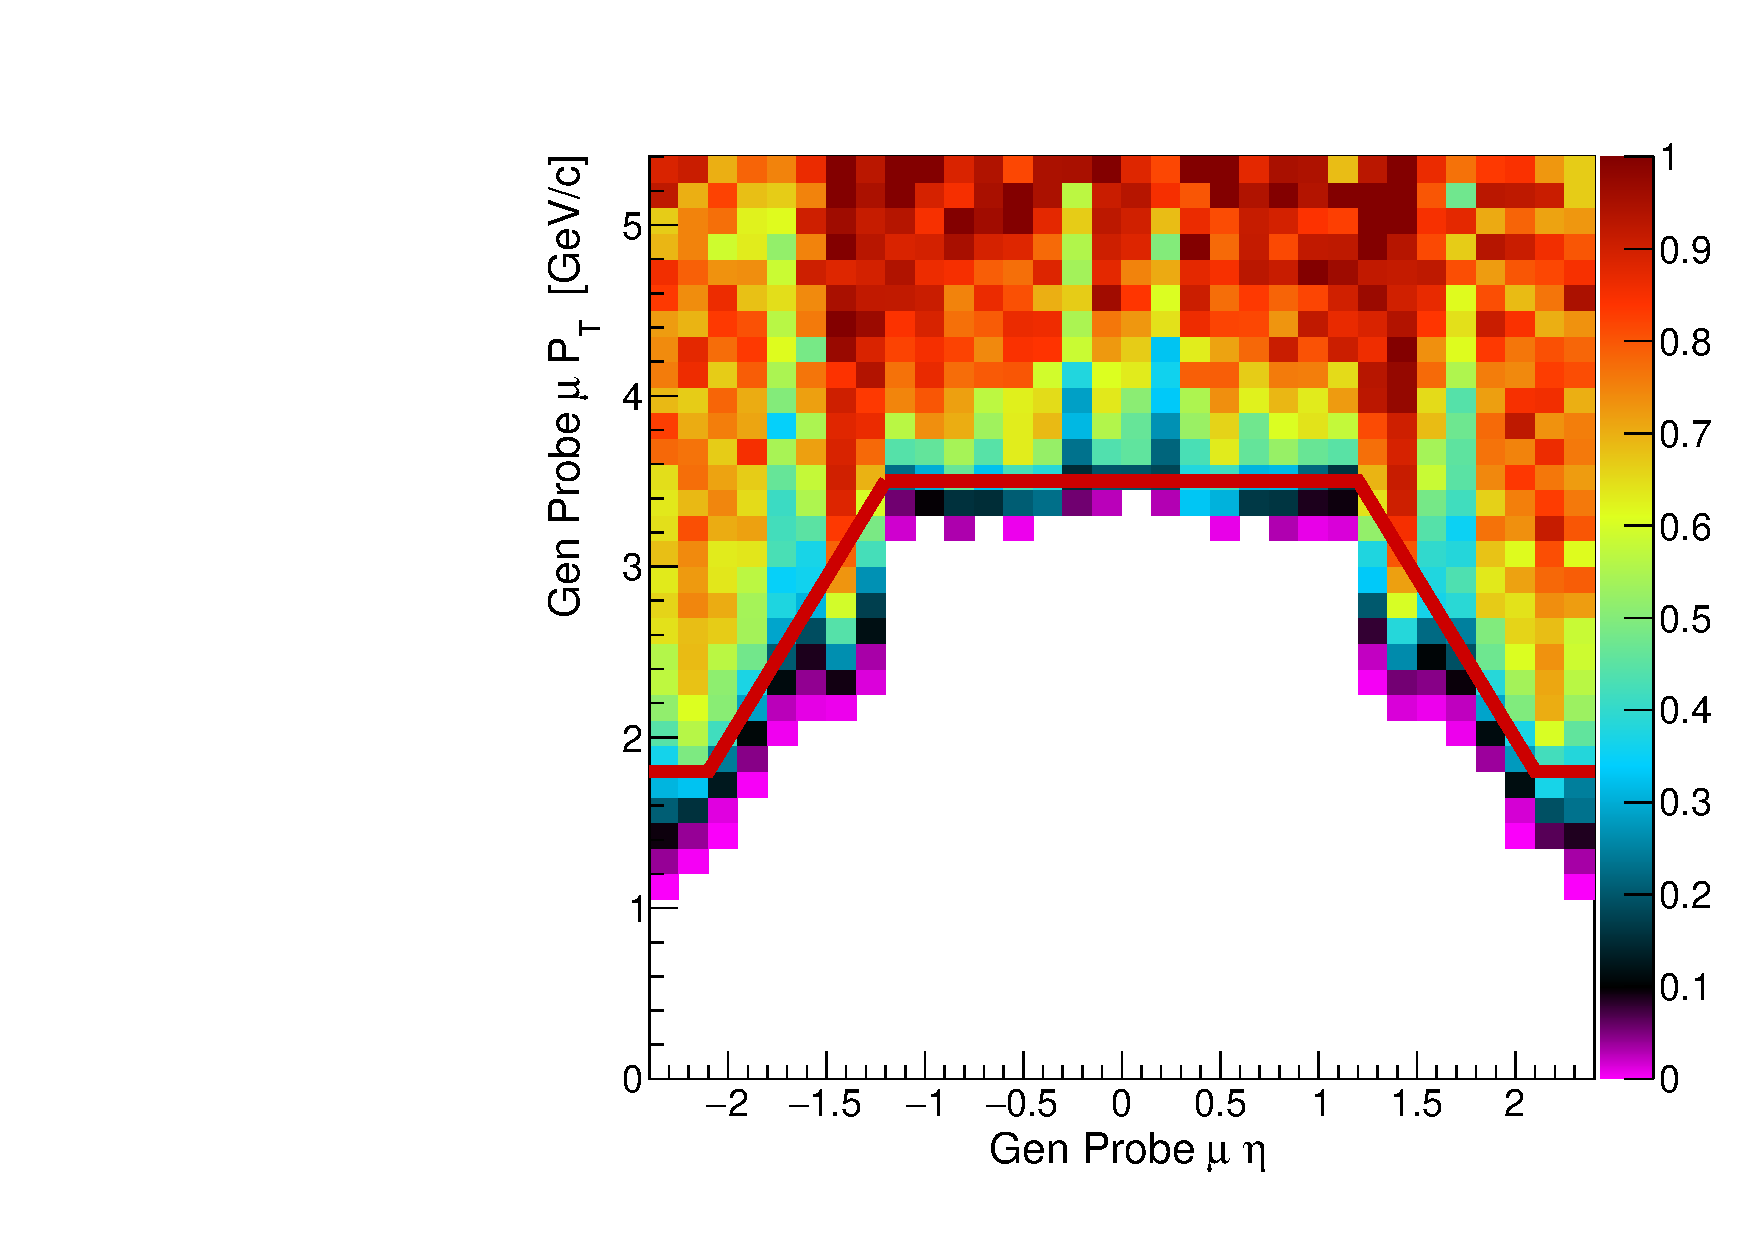
\includegraphics[width=0.48\textwidth]{Figures/Charmonia/Analysis/EventSelection/pp_AccxEff_SingleMuons}
  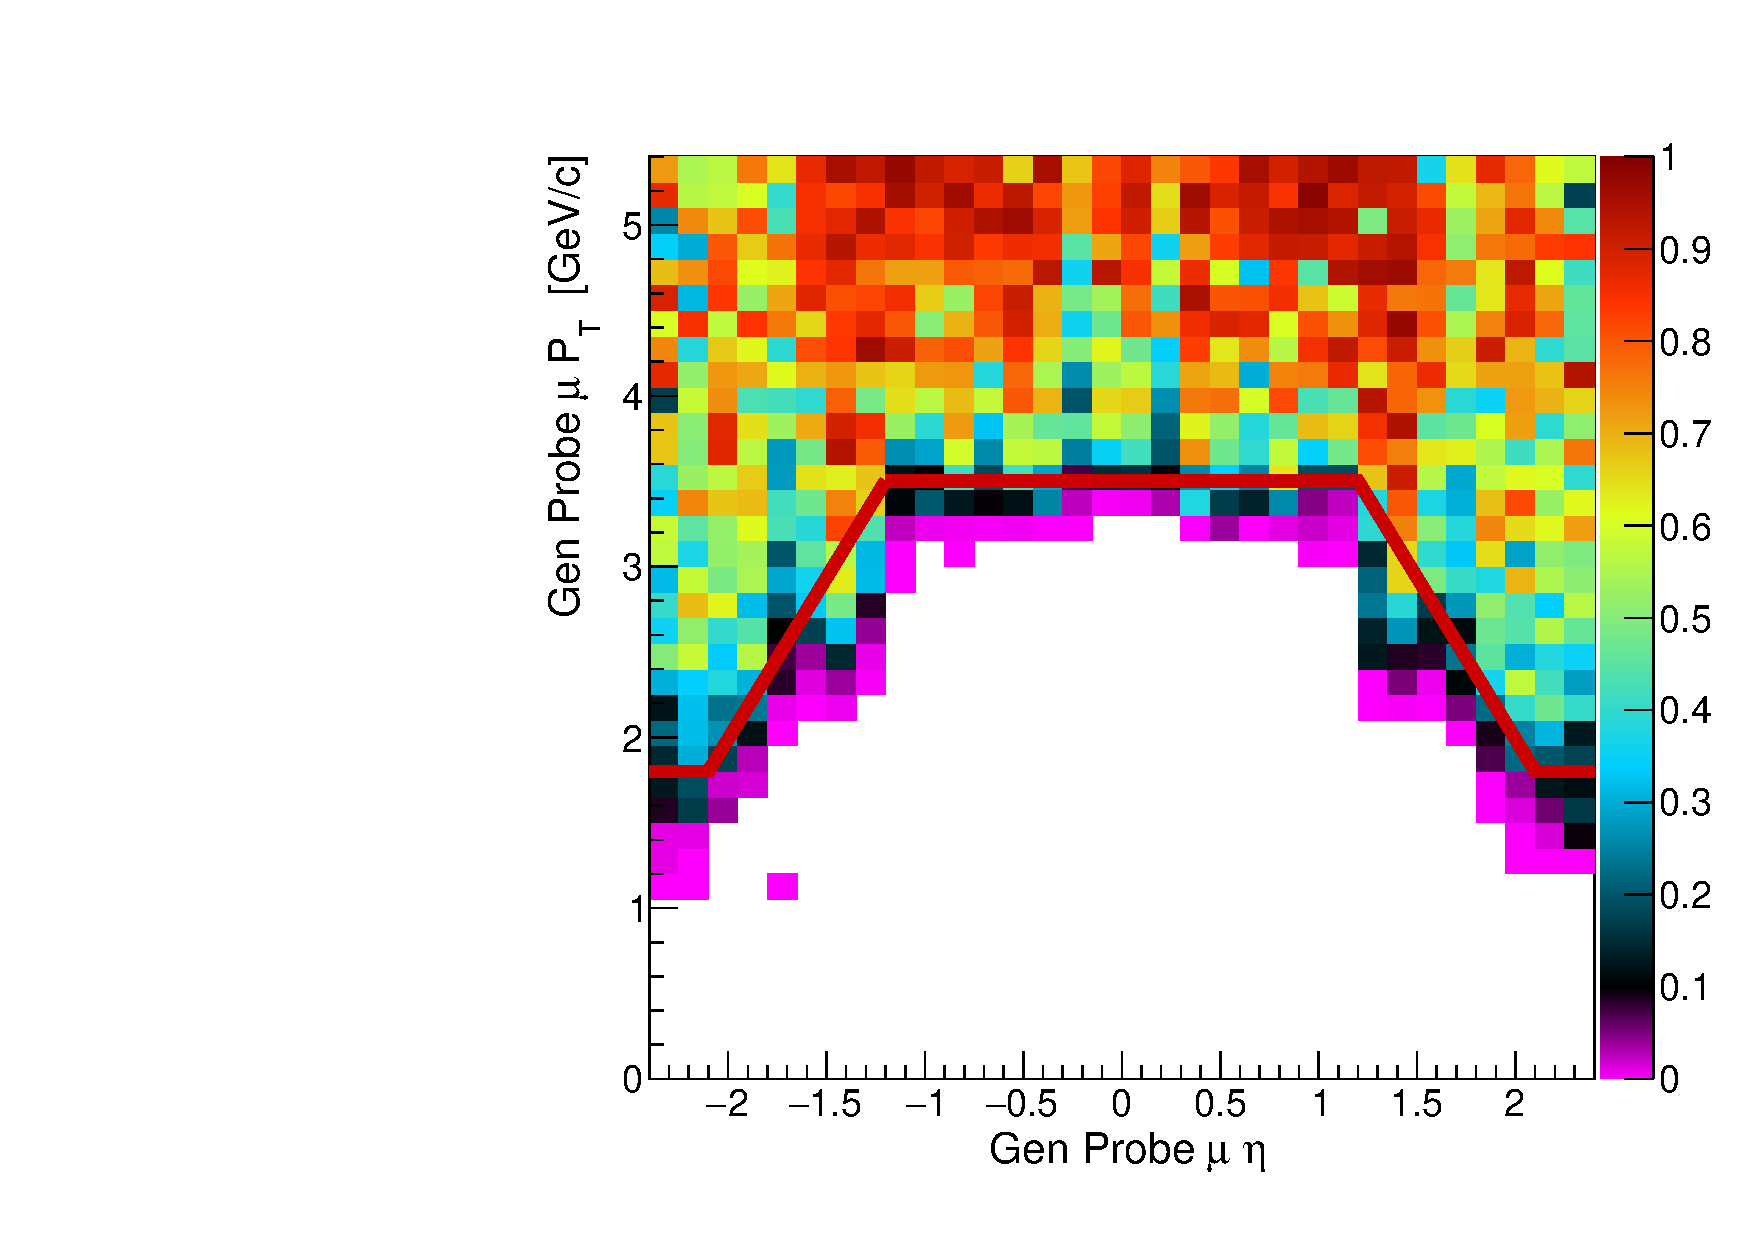
\includegraphics[width=0.48\textwidth]{Figures/Charmonia/Analysis/EventSelection/PbPb_AccxEff_SingleMuons} 
 \caption{Distribution of the ratio of the number of reconstructed, identified and triggered muons over the number of generated muons, as a function of muon \pt and $\eta$. The results are derived from the prompt \JPsi simulations corresponding to \Runpp (left) and \RunPbPb (right) collisions. The red line represents the single muon kinematic cuts.}
 \label{fig:SingleMuonAccEff}
\end{figure}


%%------------------------------------------------------------%%
\subsubsection{Charmonium selection} \label{sec:Charmonia_Analysis_Selection_CharmoniumSelection}

The \JPsiToMuMu and \PsiPToMuMu candidate selection consists of the detection of two low-\pt muons of opposite electric charge, each passing all identification criteria explained in \sect{sec:Charmonia_Analysis_Selection_MuonIdentification}, the kinematic cuts detailed in \sect{sec:Charmonia_Analysis_Selection_MuonKinematic}, and the trigger matching condition mentioned in \sect{sec:Charmonia_Analysis_Selection_Trigger}. Moreover, each dimuon candidate is required to have a $\chi^2$ probability larger than $1\%$ that the two muons derive from a common vertex. This selection is used in most CMS quarkonium analyses to remove a large fraction of background events while keeping, by construction, 99\% of signal events (two muons coming from the same vertex).


% END OF SUBSECTION
